\documentclass{beamer}
% \usetheme{metropolis}
\usefonttheme{structuresmallcapsserif}
\usepackage{times}

\title{Linear Regression: Introduction \& Estimation}
\author{Connor K. Brubaker}
\institute{
Department of Statistics \\
Texas A\&M University
}
\date{}

\begin{document}
\maketitle

\begin{frame}{Equation of a Line}
    The equation of a straight line is 
    \begin{equation*}
        y = bx + a
    \end{equation*}
    where $b$ is the slope of the line and $a$ is the intercept.
\end{frame}

\begin{frame}{Linear Relationships}
    Below are examples of \textit{perfect} linear relationships.
    \begin{center}
        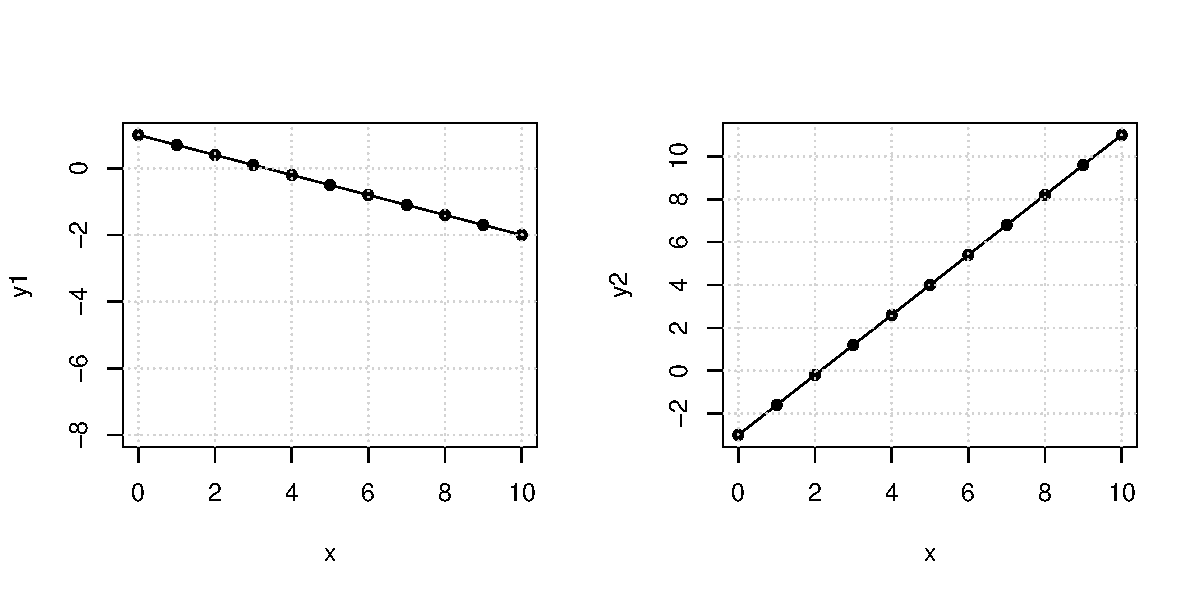
\includegraphics[width=\linewidth]{figures/perfect_linear.pdf}
    \end{center}
\end{frame}

\begin{frame}{Interpretation of slope}
    For any two points $(x_1, y_1)$ and $(x_2, y_2)$,
    \begin{equation*}
        b = \frac{y_2 - y_1}{x_2 - x_1}.
    \end{equation*}
    The slope is the \textbf{exact} rate of change in $y$ for every unit increase in $x$.
\end{frame}

\begin{frame}{Interpretation of intercept}
    When $x = 0$,
    \begin{equation*}
        y = b(0) + a = a
    \end{equation*}
    The intercept is the \textbf{exact} value of $y$ when $x = 0$. 
\end{frame}

\begin{frame}{Example: Housing Prices}
    \begin{itemize}[<+->]
        \item How much should you pay for a house?
        \item Factors that influence price:
        \begin{itemize}
            \item Location
            \item Year built
            \item Amenities
            \item \textbf{Square footage}
        \end{itemize}
        \item To determine a price, we might \textbf{model} price as a function of square footage:
        \begin{equation*}
            \textrm{Price} = f(\textrm{Square Footage}) + \varepsilon
        \end{equation*}
        $f$ is called the \textbf{regression function}.
    \end{itemize}
\end{frame}

\begin{frame}{Motivating Example: Housing Prices}
    Scatter plots help determine the functional relationship between two variables.
    \begin{center}
        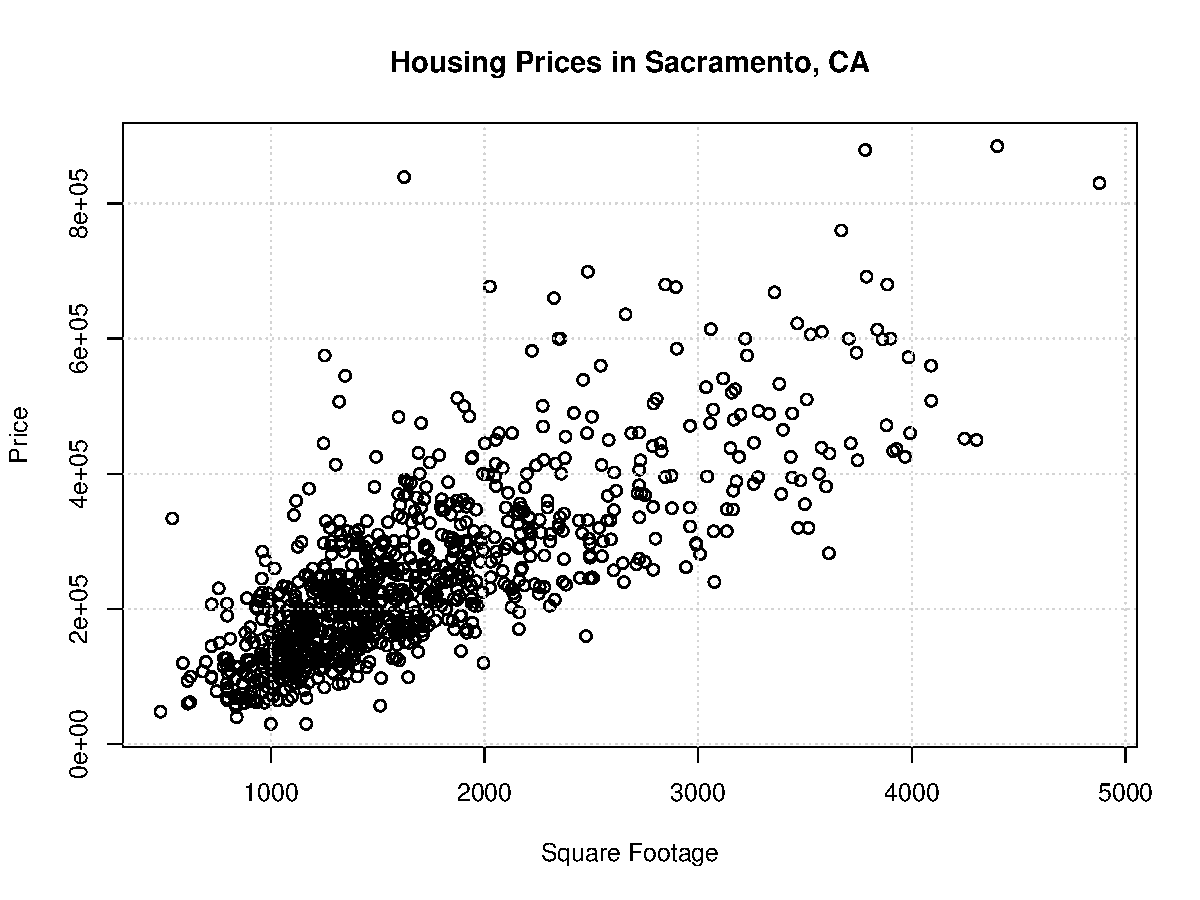
\includegraphics[width=.85\linewidth]{figures/sacramento.pdf}
    \end{center}
\end{frame}

\begin{frame}{Simple Linear Regression}
    The simplest model is where $f$ is a linear function:
    \begin{equation*}
        f(x) = \beta_0 + \beta_1 x.
    \end{equation*}
    The model becomes 
    \begin{equation*}
        Y_i = \beta_0 + \beta_1 X_i + \varepsilon_i.
    \end{equation*}
    \begin{equation*}
        \textrm{Price}_i = \beta_0 + \beta_1 \textrm{Square Footage}_i + \varepsilon_i.
    \end{equation*}
    $Y_i$ is called the \textbf{dependent variable} or the \textbf{response} and $X_i$ is called the \textbf{independent variable} or \textbf{predictor}.
\end{frame}

\begin{frame}{Parameters of SLR}
    Under SLR, the model is 
    \begin{equation*}
        Y_i = \beta_0 + \beta_1 X_i + \varepsilon_i.
    \end{equation*}
    The \textbf{parameters} of the model are the intercept $\beta_0$ and the slope $\beta_1$. These are unknown and must be estimated using data.
\end{frame}

\begin{frame}{The Error Term}
    Under SLR, the model is 
    \begin{equation*}
        Y_i = \beta_0 + \beta_1 X_i + \varepsilon_i.
    \end{equation*}
    The \textbf{error term} $\varepsilon_i$ accounts for the fact that 
    \begin{itemize}
        \item not all the points lie exactly on the regression line and
        \item $Y$ cannot be perfectly predicted from $X$ alone
    \end{itemize}
\end{frame}

\begin{frame}{The Error Term}
    Under SLR, the model is 
    \begin{equation*}
        Y_i = \beta_0 + \beta_1 X_i + \varepsilon_i.
    \end{equation*}
    We assume the \textbf{error term} $\varepsilon_i$ satisfies
    \begin{itemize}
        \item $\varepsilon_i \sim \mathcal{N}(0, \sigma^2)$
        \item the error terms are all independent of each other (mutually independent)
    \end{itemize}
\end{frame}

\begin{frame}{Regression Models the Conditional Expectation}
    In SLR, $\varepsilon_i \sim \mathcal{N}(0, \sigma^2)$ so that $\mathbb{E}(\varepsilon_i) = 0$. Treating $X_i$ as a given constant, we have  
    \begin{equation*}
        \begin{split}
            \mathbb{E}[Y_i | X_i] &= \mathbb{E}(\beta_0 + \beta_1 X_i + \varepsilon_i) \\
            &= \beta_0 + \beta_1 X_i + \mathbb{E}(\varepsilon_i) \\
            &= \beta_0 + \beta_1 X_i
        \end{split}
    \end{equation*}
    $\mathbb{E}[Y_i | X_i]$ is the conditional expectation of $Y_i$ given $X_i$ - it \textit{depends} on the value $X_i$. 
\end{frame}

\begin{frame}{Line of Best Fit}
    Many different lines ``fit'' the data, which is the best?
    \begin{center}
        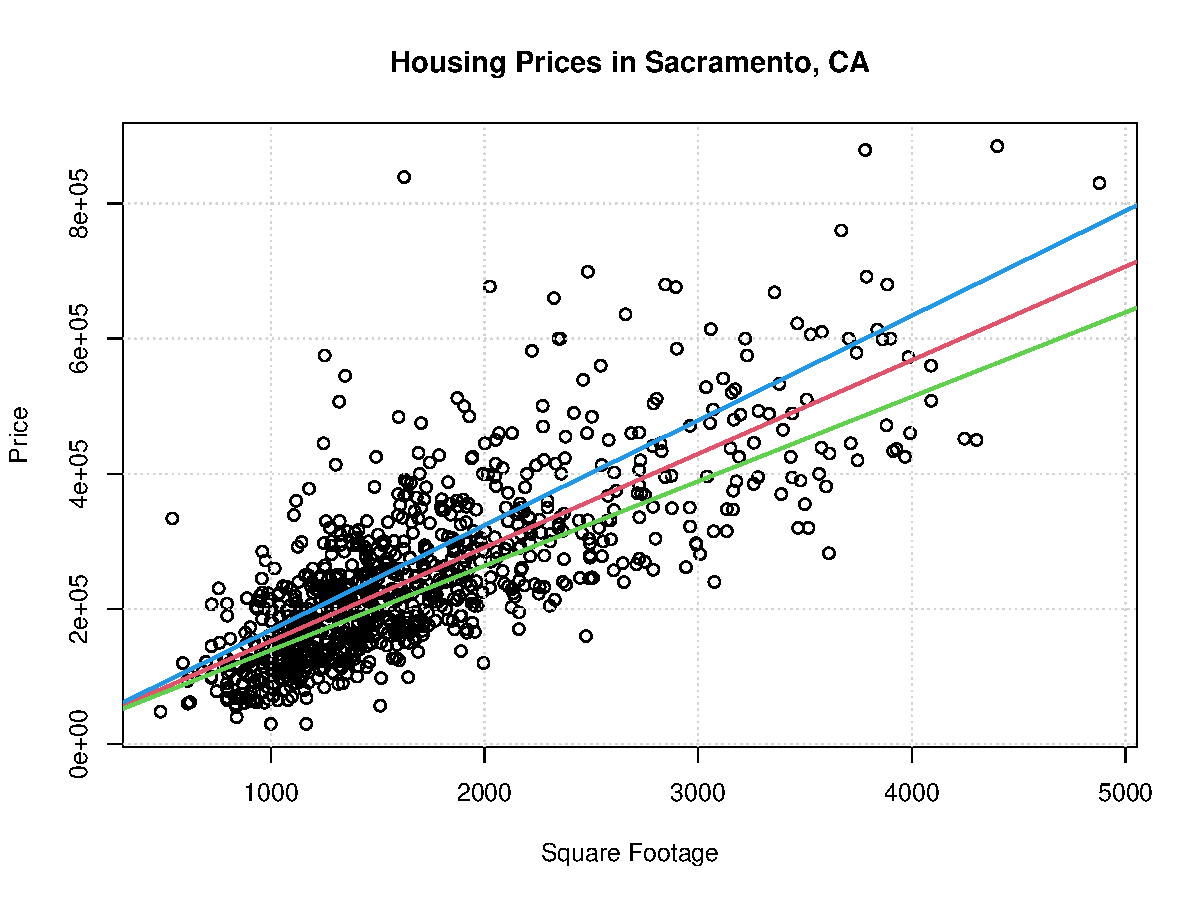
\includegraphics[width=.9\linewidth]{figures/sacramento_lines.pdf}
    \end{center}
\end{frame}

\begin{frame}{Residuals}
    Given some $\beta_0$ and $\beta_1$, the predicted value of $Y_i$ at $X_i$ is 
    \begin{equation*}
        \hat{Y}_i = \beta_0 + \beta_1 X_i
    \end{equation*}
    The $i$th residual is 
    \begin{equation*}
        \hat{\varepsilon}_i = Y_i - \hat{Y}_i = Y_i - \beta_0 - \beta_1 X_i
    \end{equation*}
\end{frame}

\begin{frame}{Least Squares Criterion}
    We choose the line with intercept $\beta_0$ and slope $\beta_1$ that minimizes the sum of squared residuals, 
    \begin{equation*}
        RSS = \sum_{i=1}^n \hat{\varepsilon}_i^2 = \sum_{i=1}^n (Y_i - \beta_0 - \beta_1 X_i)^2
    \end{equation*}
    The values of $\beta_0$ and $\beta_1$ that minimize $RSS$ are called the \textbf{least squares estimators}.
\end{frame}

\begin{frame}{Residuals of the Housing Data}
    \begin{center}
        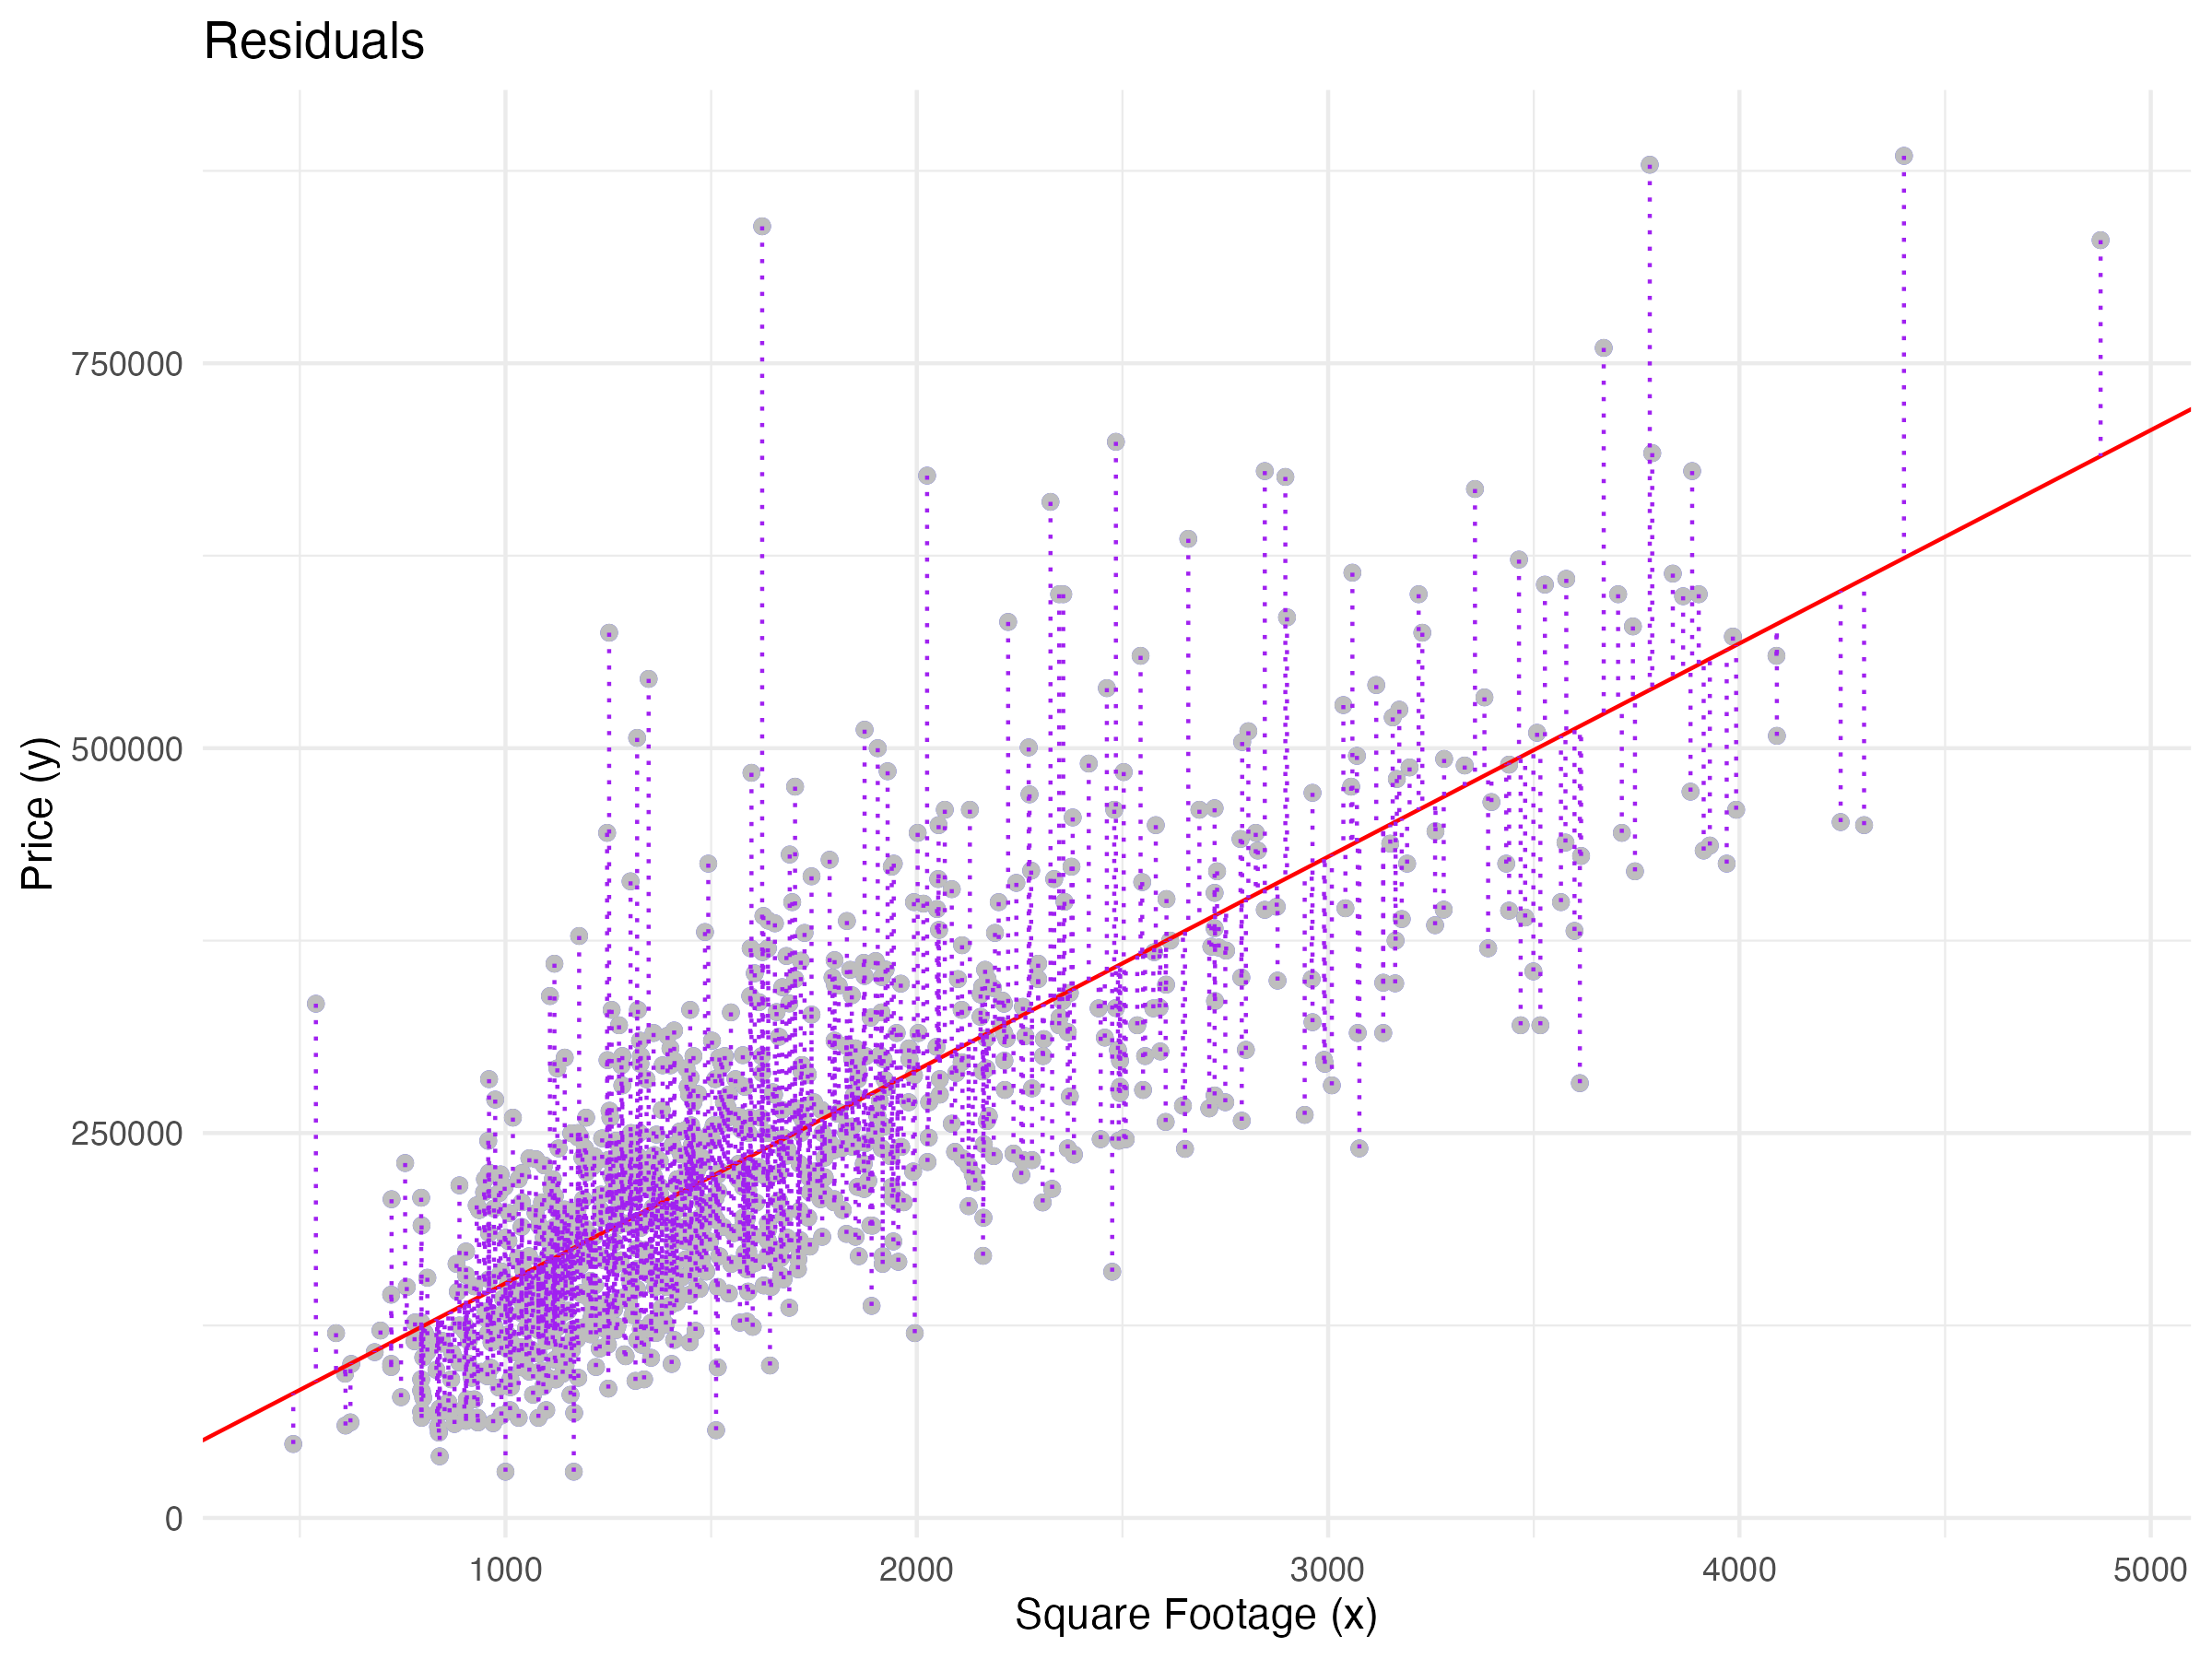
\includegraphics[width=.9\linewidth]{figures/housing_resid.png}
    \end{center}
\end{frame}

\begin{frame}[t]{Least Squares Estimators}
    Use principles of calculus to find the minimizers of the residual sum of squares,
    \begin{equation*}
        RSS = \sum_{i=1}^n (Y_i - \beta_0 - \beta_1 X_i)^2.
    \end{equation*}
\end{frame}

\begin{frame}{Least Squares Estimators}
    Define 
    \begin{equation*}
        SXY = \sum_{i=1}^n (X_i - \bar{X})(Y_i - \bar{Y})\ \ \textrm{and}\ \ SXX = \sum_{i=1}^n (X_i - \bar{X})^2.
    \end{equation*}
    The least squares estimators are 
    \begin{equation*}
        \hat{\beta}_1 = \frac{SXY}{SXX}\ \ \textrm{and}\ \ \hat{\beta}_0 = \bar{Y} - \hat{\beta}_1 \bar{X}.
    \end{equation*}
\end{frame}

\begin{frame}{Covariance}
    The quantity 
    \begin{equation*}
        SXY = \sum_{i=1}^n (X_i - \bar{X})(Y_i - \bar{Y})
    \end{equation*}
    is an estimator of the \textbf{covariance} between $X$ and $Y$.
\end{frame}

\begin{frame}{Covariance}
    The covariance $Cov(X, Y)$ between $X$ and $Y$ 
    \begin{itemize}
        \item quantifies the strength of the linear relationship between $X$ and $Y$,
        \item can be positive or negative, and
        \item could be near zero if the relationship is non-linear.
    \end{itemize}
\end{frame}

\begin{frame}{Covariance}
    \begin{center}
        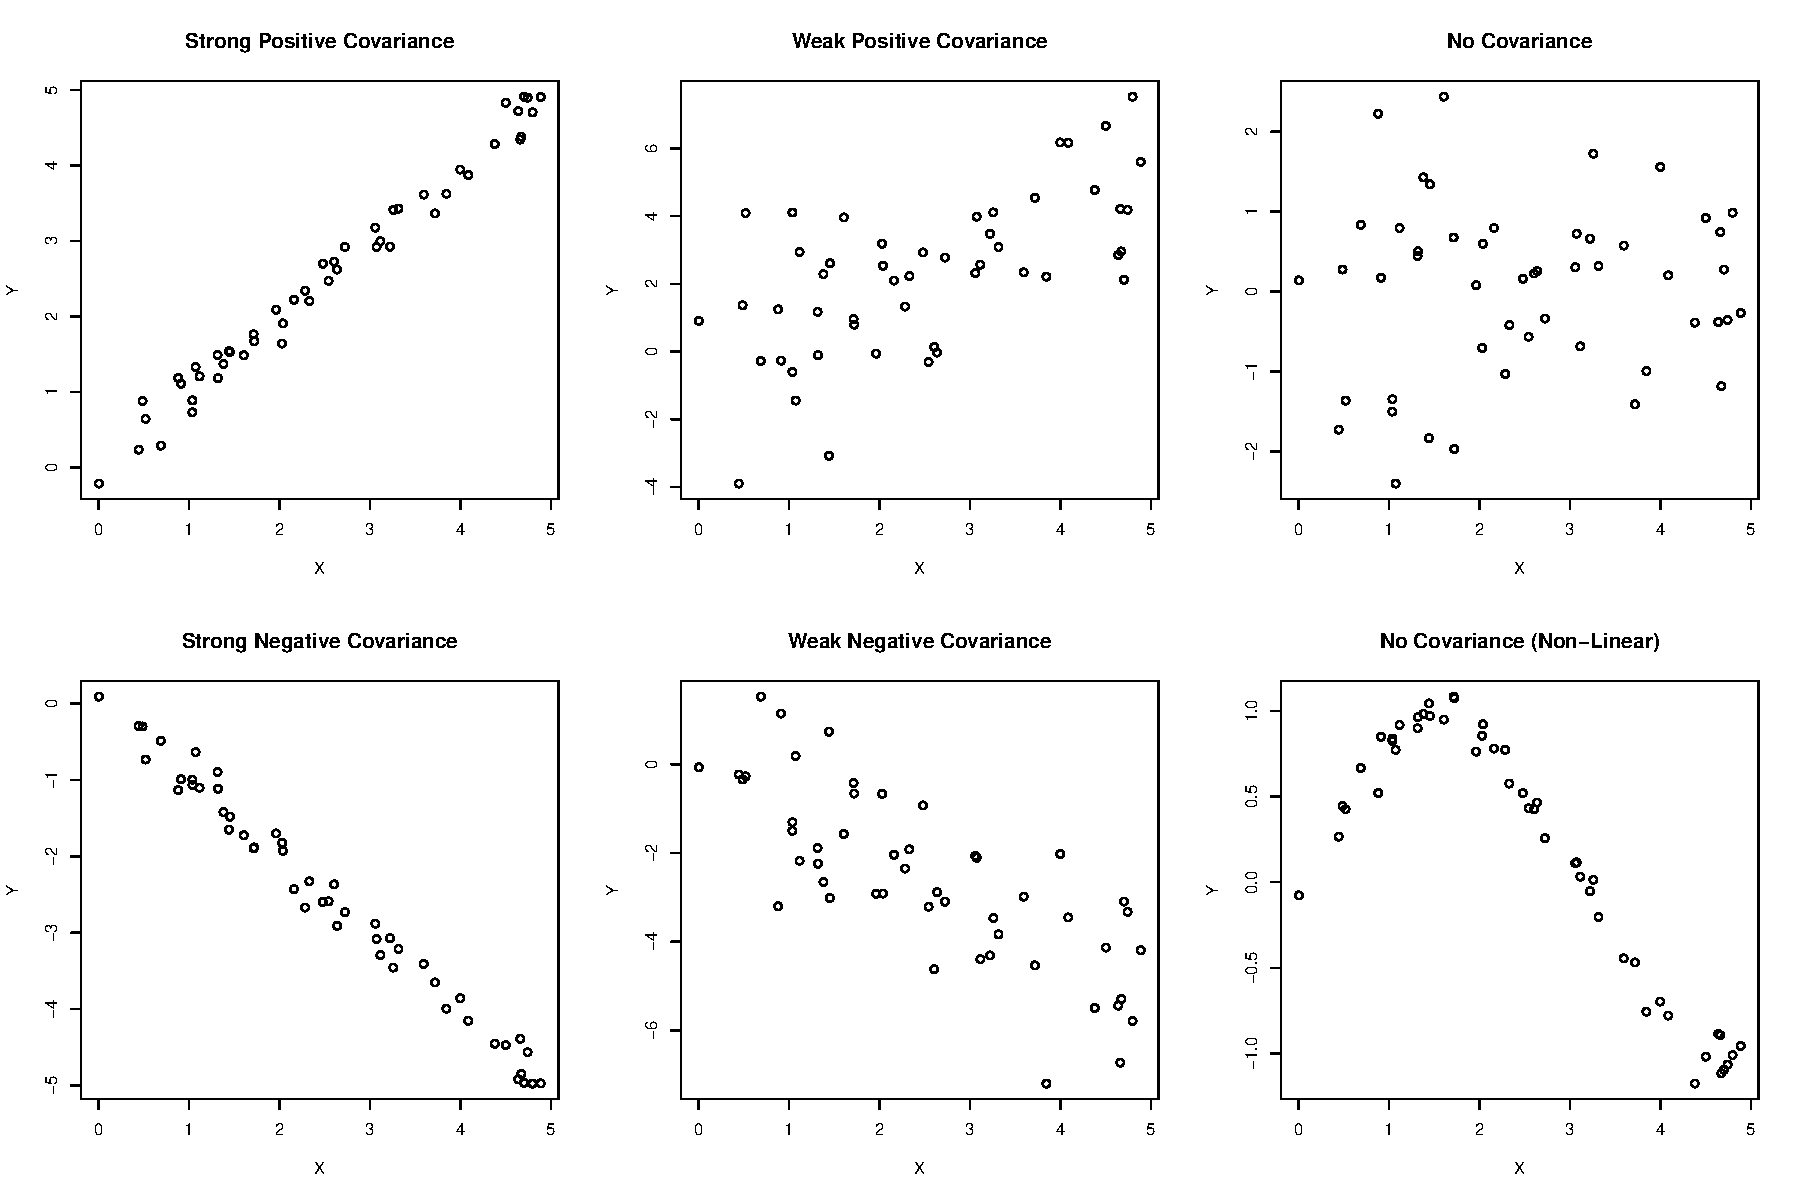
\includegraphics[width=\linewidth]{figures/covariance.pdf}
    \end{center}
\end{frame}

\begin{frame}{Correlation}
    Standardizing the covariance gives the correlation $\rho$:
    \begin{equation*}
        \rho = \frac{Cov(X, Y)}{\sigma_X \sigma_Y}
    \end{equation*} 
    It has the same interpretation but is restricted to lie between $-1$ and $1$. Correlation of $1$ is a perfect positive linear relationship.
\end{frame}

\begin{frame}{Interpretation of Slope Parameter}
    Recall 
    \begin{equation*}
        \mathbb{E}[Y_i | X_i] = \beta_0 + \beta_1 X_i
    \end{equation*}
    \begin{itemize}
        \item The slope is the change in the \textit{expected value} of $Y$ for every unit increase in $X$. 
        \item The intercept is the \textit{expected value} of $Y$ when $X = 0$.
    \end{itemize}
\end{frame}

\begin{frame}{Example: Housing Prices}
    \begin{columns}
        \begin{column}{0.5\linewidth}
            For the housing data, 
            \begin{equation*}
                \hat{\beta_0} = 13859.393
            \end{equation*}
            and 
            \begin{equation*}
                \hat{\beta}_1 = 138.546
            \end{equation*}
        \end{column}
        \begin{column}{0.5\linewidth}
            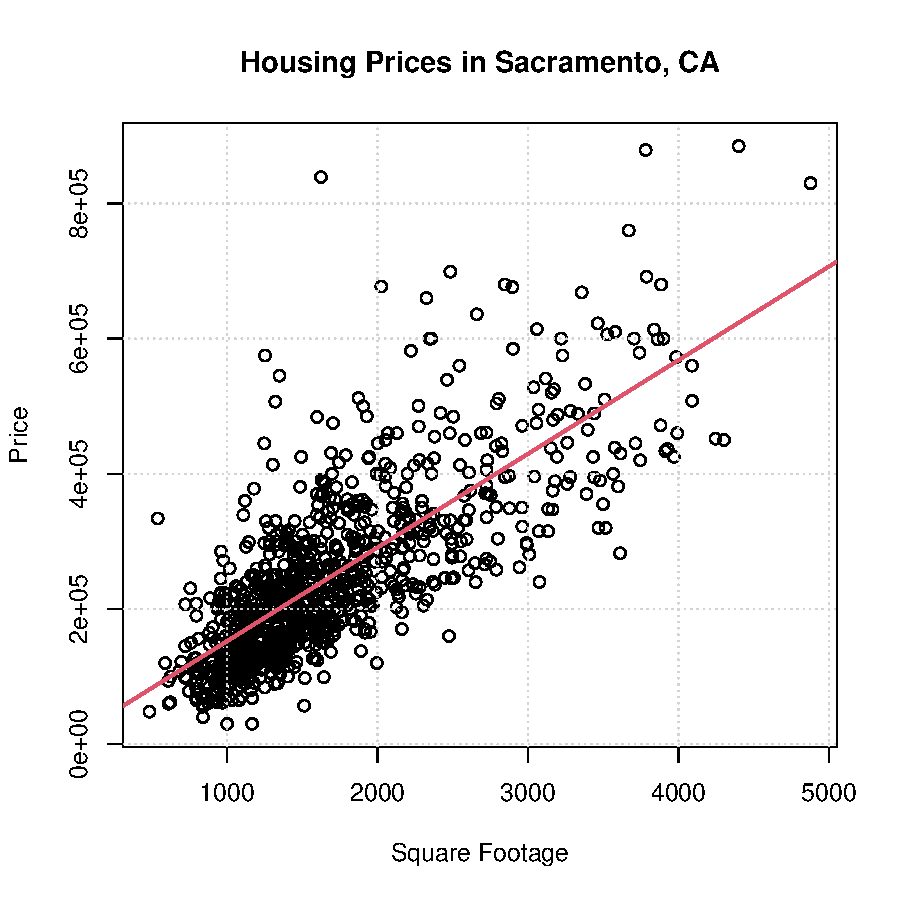
\includegraphics[width=\linewidth]{figures/sacramento_ls.pdf}
        \end{column}
    \end{columns}
\end{frame}

\begin{frame}{No Intercept Model}
    Sometimes it is appropriate to fit the SLR model with no intercept:
    \begin{equation*}
        Y_i = \beta_1 X_i + \varepsilon_i
    \end{equation*}
    Is this appropriate for the housing data?
\end{frame}

\begin{frame}{Linear Model in R}
    A linear model can be fit using
    \vspace*{0.5em}

    \footnotesize
    \texttt{> model <- lm(price $\sim$ sqft)} \par
    \texttt{> model <- lm(price $\sim$ sqft - 1) \# no intercept} \par
    \texttt{> summary(model)} \par 
\end{frame}

\begin{frame}{Linear Model in R}
    \begin{center}
        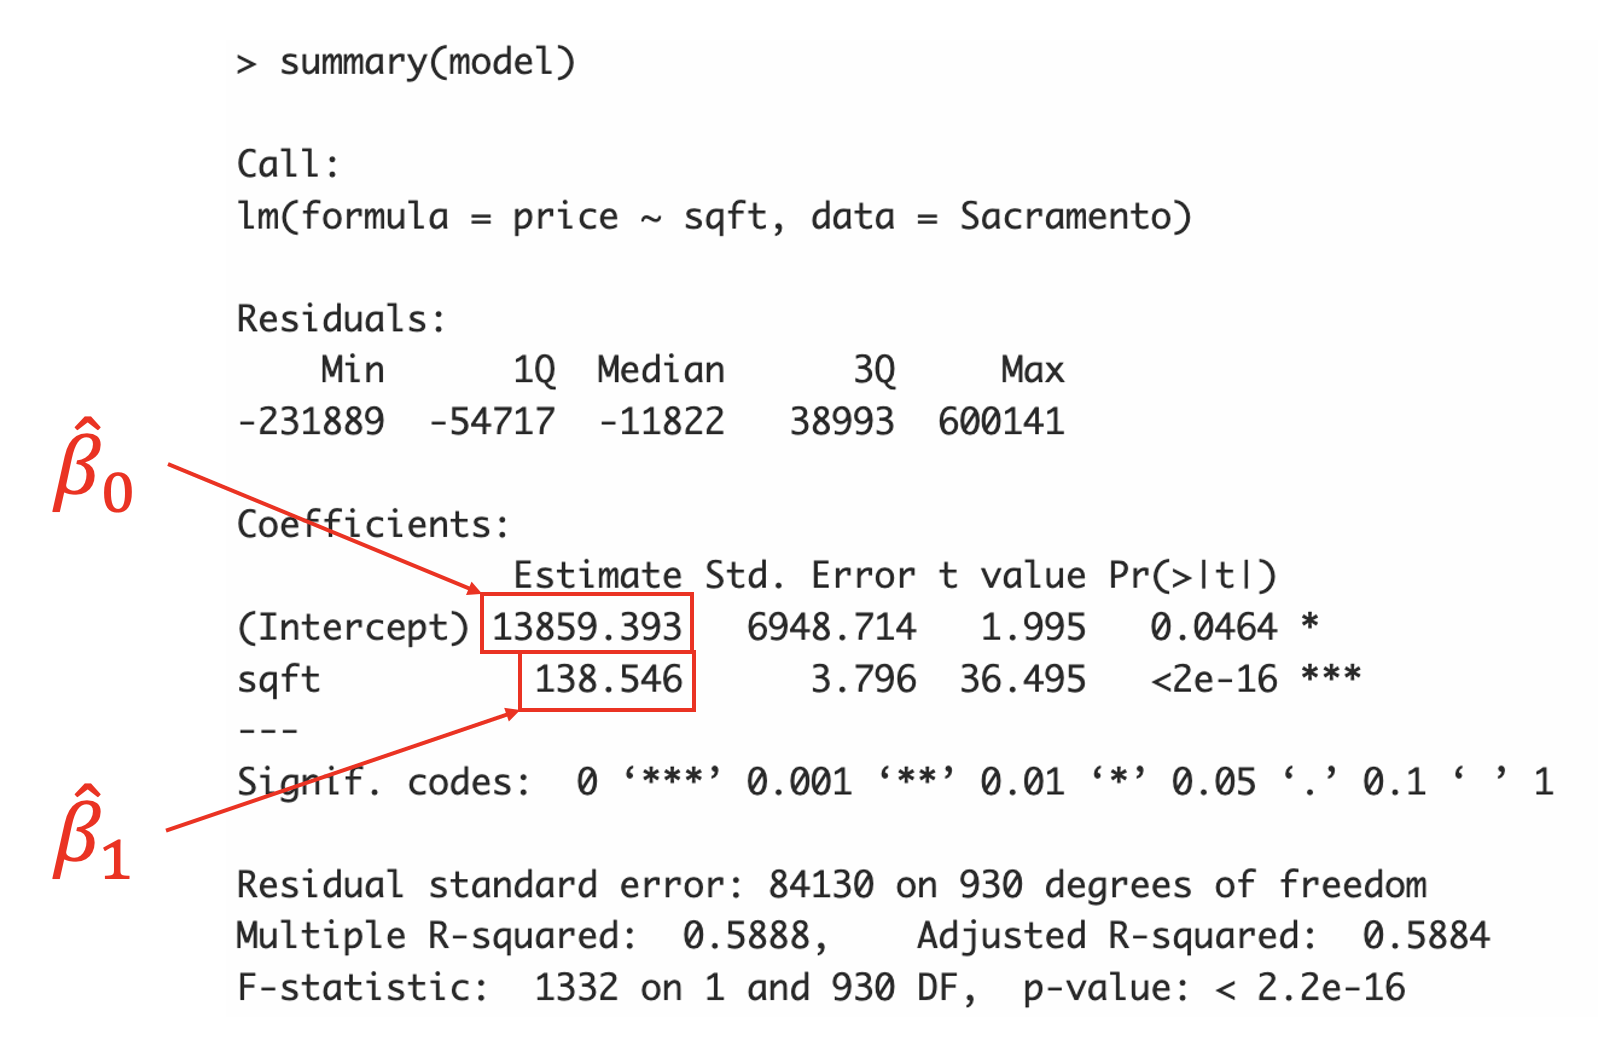
\includegraphics[width=.9\linewidth]{figures/summary_estimates.png}
    \end{center}
\end{frame}

\begin{frame}{Association and Causation}
    \textbf{A strong relationship between two variables does not always imply a causal relationship.}

    \vspace*{1em}
    A strong association between two variables is often due to lurking variables that we are not aware of. 
\end{frame}

\begin{frame}{Association and Causation}
    \begin{center}
        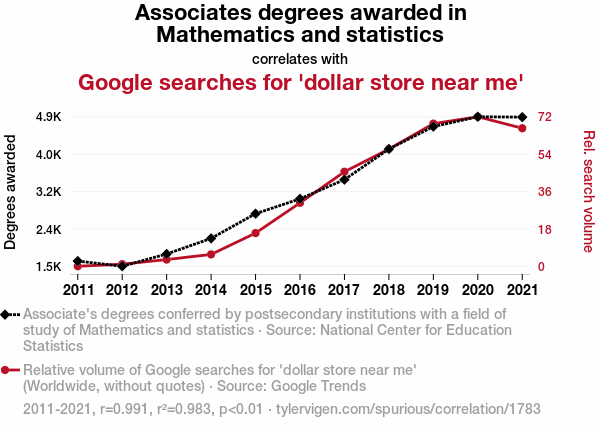
\includegraphics[width=.8\linewidth]{figures/1783_associates-degrees-awarded-in-mathematics-and-statistics_correlates-with_google-searches-for-dollar-store-near-me.png}
    \end{center}
    \footnotesize 
    \href{https://www.tylervigen.com/spurious-correlations}{https://www.tylervigen.com/spurious-correlations}
\end{frame}

\begin{frame}{Association and Causation}
    \begin{itemize}
        \item The best evidence for causal relationships comes from properly designed randomized experiments. 
        \item Observational studies can show a strong association, but it is not appropriate to conclude causation.
    \end{itemize}
\end{frame}

\begin{frame}{Does Smoking Cause Lung Cancer?}
    \begin{itemize}
        \item Unethical to investigate this with an experiment.
        \item Observational studies have demonstrated an association between lung cancer and smoking.
        \item Evidence has been collected from many studies.
        \item It is plausible that smoking causes cancer, but the conclusion is not as strong as evidence from a randomized experiment. 
    \end{itemize}
\end{frame}

\end{document}